\subsection{Замкнутая трофическая цепь}
    \subsubsection{Равновесные состояния}
        Аналогично незамкнутой системе, в системе с частичным восстановлением ресурса (\ref{cycle}) при \(Q > 0\) могут существовать \( n \) равновесных состояний типа \(\left[ N_0, N_1, \ldots, N_q, 0, \ldots, 0 \right]\), которые могут быть найдены из уравнений
        \begin{equation} \label{cycle_stationary_equations}
            \frac{dN}{dt} = 0 \Rightarrow
            \left\lbrace\begin{split}
                & Q + \sum_{i=1}^{q} a_i m_i N_i = \alpha_0 N_0 N_1, \\
                & \alpha_i N_{i+1} = k_i \alpha_{i-1} N_{i-1} - m_i, \quad i=\overline{1,q}                
            \end{split}\right.
        \end{equation}

        Поскольку связь \(N_{i-1}\) и \(N_{i+1}\) точно такая же, что и у незамкнутой модели, то значения \(N_i\) также могут быть определены по формулам (\ref{flow_2s}, \ref{flow_2s1}). Остаётся найти явные выражения для \(N_0\) и \( N_1\).
        
        Используем обозначения (\ref{flow_sub}) и введём новые:
        \begin{equation}
            \begin{split}
            & \varphi_s = \sum_{j=1}^{s} a_{2j} m_{2j} H_{2s-1}, \quad 
            \psi_s = \sum_{j=1}^{s} a_{2j-1} m_{2j-1} H_{2s-2}, \\
            & \sigma_i = \sum_{j=1}^{i} a_j m_j f_{j-1} H_{j-1} \quad (H_0 = 1, \, f_0 = 0).
            \end{split}
        \end{equation}

        \begin{enumerate}
            \item Пусть \(q = 2s\) -- \textit{чётное}. Тогда аналогично шагам для незамкнутой цепи получаем \( N_1 = f_{2s} \).
            Используя первое уравнение в (\ref{cycle_stationary_equations}), будем иметь            
            \begin{equation*}
            \begin{split}
                & Q + \sum\limits_{i=1}^{s} a_{2i-1} m_{2i-1} H_{2i-2}(N_1 - f_{2i-2}) + \sum\limits_{i=1}^{s} a_{2i} m_{2i} H_{2i-1}(N_0-f_{2i-1}) = \alpha_0 N_0 N_1, \\
                & Q + \sum\limits_{i=1}^{s} a_{2i-1} m_{2i-1} H_{2i-2}(f_{2s} - f_{2i-2})  = \alpha_0 N_0 N_1 - \sum\limits_{i=1}^{s} a_{2i} m_{2i} H_{2i-1}(N_0-f_{2i-1}), \\
                & Q + f_{2s} \sum\limits_{i=1}^{s} a_{2i-1} m_{2i-1} H_{2i-2} - \sum\limits_{i=1}^{s} a_{2i-1} m_{2i-1} H_{2i-2} f_{2i-2} = \\
                & = N_0 \left( \alpha_0 f_{2s} - \sum\limits_{i=1}^{s} a_{2i} m_{2i} H_{2i-1} \right) + \sum\limits_{i=1}^{s} a_{2i} m_{2i} H_{2i-1} f_{2i-1},  \\
                & Q + f_{2s} \psi_s - \sigma_{2s} = N_0 \left( \alpha_0 f_{2s} - \varphi_s \right), \\
                & N_0 = \frac{Q + f_{2s} \psi_s - \sigma_{2s}}{\alpha_0 f_{2s} - \varphi_s}.
            \end{split}
            \end{equation*}

            \item Пусть \(q = 2s+1\) -- \textit{нечётное}. Тогда \( N_1 = f_{2s+1} \) и
            \begin{equation*}
                \begin{split}
                    & Q + \sum\limits_{i=1}^{s+1} a_{2i-1} m_{2i-1} H_{2i-2}(N_1 - f_{2i-2}) + \sum\limits_{i=1}^{s} a_{2i} m_{2i} H_{2i-1}(N_0-f_{2i-1}) = \alpha_0 N_0 N_1, \\
                    & Q + \sum\limits_{i=1}^{s} a_{2i} m_{2i} H_{2i-1}(f_{2s+1} - f_{2i-1})  = \alpha_0 N_0 N_1 - \sum\limits_{i=1}^{s+1} a_{2i-1} m_{2i-1} H_{2i-2}(N_1 - f_{2i-2}), \\
                    & Q + f_{2s+1} \sum\limits_{i=1}^{s} a_{2i} m_{2i} H_{2i-1} - \sum\limits_{i=1}^{s} a_{2i} m_{2i} H_{2i-1} f_{2i-1} = \\
                    & = N_1 \left( \alpha_0 f_{2s+1} - \sum\limits_{i=1}^{s+1} a_{2i-1} m_{2i-1} H_{2i-2} \right) + \sum\limits_{i=1}^{s+1} a_{2i-1} m_{2i-1} H_{2i-2} f_{2i-2},  \\
                    & Q + f_{2s+1} \varphi_s - \sigma_{2s+1} = N_1 \left( \alpha_0 f_{2s+1} - \psi_{s+1} \right), \\
                    & N_0 = \frac{Q + f_{2s+1} \varphi_s - \sigma_{2s+1}}{ \alpha_0 f_{2s+1} - \psi_{s+1} }.
                \end{split}
                \end{equation*}
        \end{enumerate}

        Очевидно, что стационарные значения численностей \(N_i\) имеют смысл, только когда они положительные.

    %     \begin{statement}
    %         Если в трофической цепи длины \(q\) численность \(N_q > 0\), то \(N_i > 0 \, (i=\overline{1,q-1})\).
    %     \end{statement}

    %     \begin{proof}
    %         Для начала заметим, что \(f_{2s}\) и \(f_{2s+1}\) положительны и монотонно возрастают с увеличением \(s\). Величины \(N_0\) и \(N_1\) также положительны и зависят от параметра \(q\) -- длины трофической цепи.  
    %         Поскольку все параметры положительные, то численность \( N_{q-1} > 0 \).

    %         Из условия \( N_q > 0 \) и (\ref{cycle_2s}, \ref{cycle_2s1}) получим неравенство
    %         \begin{equation} \label{cycle_lower}
    %             Q > \alpha_0 f_{q-1} f_{q}
    %         \end{equation} 

    %         Предположим противное: \(\exists p < q : N_p \leq 0\). Возможны 4 варианта: \(p\) и \(q\) одинаковой чётности и разной чётности.

    %         \begin{enumerate}
    %             \item Пусть \(q = 2s \) и \( N_0 = \frac{Q}{\alpha_0 f_{2s}}, N_1 = f_{2s}\).
    %             \begin{enumerate}
    %                 \item \(p = 2u \, (u < s)\), тогда из (\ref{cycle_2s}) следует, что \( N_p = N_{2u} \leq 0 \), если \(N_0 \leq f_{2u-1}\). Значит \(Q \leq \alpha_0 f_{2u-1} f_{2s} \). Сравнивая с (\ref{cycle_lower}) получаем
    %                 \begin{equation*}
    %                     \alpha_0 f_{2s-1} f_{2s} < Q \leq \alpha_0 f_{2u-1} f_{2s} \Rightarrow f_{2s-1} < f_{2u-1}.
    %                 \end{equation*}
    %                 Это невозможно, поскольку \(f_{2s-1}\) монотонно возрастает с ростом \(s\).

    %                 \item \(p = 2u+1 \, (2u < 2s-1)\), тогда из (\ref{cycle_2s1}) следует, что \( N_p = N_{2u+1} \leq 0 \) при \(N_1 \leq f_{2u}\), т.е. \(f_{2s} \leq f_{2u} \). Что также невозможно из-за монотонного возрастания \(f_{2s}\) с ростом \(s\). 
    %             \end{enumerate}

    %             \item Пусть \( q = 2s+1 \) и \( N_0 = f_{2s+1}, N_1 = \frac{Q}{\alpha_0 f_{2s+1}}\).
    %             \begin{enumerate}
    %                 \item \(p = 2u \, (2u-1 < 2s)\), тогда \( N_p = N_{2u} \leq 0 \) при \(N_0 \leq f_{2u-1}\). Значит \(f_{2s+1} < f_{2u-1} \). 
                    
    %                 Это невозможно, поскольку \(f_{2s-1}\) монотонно возрастает с ростом \(s\).

    %                 \item \(p = 2u+1 \, (u < s)\), тогда \( N_p = N_{2u+1} \leq 0 \) при \(N_1 \leq f_{2u}\), т.е. \( Q \leq \alpha f_{2u} f_{2s+1} \). Сравнивая с (\ref{cycle_lower}) получаем
    %                 \begin{equation*}
    %                     \alpha_0 f_{2s} f_{2s+1} < Q \leq \alpha f_{2u} f_{2s+1} \Rightarrow f_{2s} < f_{2u}.
    %                 \end{equation*}
    %                 Что также невозможно из-за монотонного возрастания \(f_{2s}\) с ростом \(s\). 
    %             \end{enumerate}
    %         \end{enumerate}
    %     \end{proof}
        
    %     \begin{corollary}
    %         Из (\ref{cycle_lower}) следует, что если длина трофической цепи равна \(q\), то скорость поступления ресурса \( Q \) должна превосходить критическое значение 
    %         \begin{equation*}
    %             Q^* (q) = \alpha_0 f_{q-1} f_{q}.
    %         \end{equation*}
    %     \end{corollary}

    %     \subsubsection{Условия существования цепи фиксированной длины}

    %     Для определения устойчивости равновесного состояния трофической цепи длины \(q\): \(N^* = [ N_0, N_1, \dots, N_q, 0, \dots, 0 ]\) будем исследовать собственные значения матрицы системы (\ref{cycle}), линеаризованной в окрестности этого состояния.
        
    %     Найдём матрицу якоби этой системы и подставим равновесную точку: \( \left.\frac{\partial f}{\partial N}\right|_{N^*} \) (\(f\) -- правая часть системы). Получим матрицу
    %     \begin{equation}
    %         J = \left\Vert \begin{matrix}
    %             A_q & 0 \\
    %             0 & D_{n-q}
    %         \end{matrix} \right\Vert,
    %     \end{equation}
    %     где \(D_{n-q} = \diag\left\{ -m_{q+1} + k_{q+1} \alpha_q N_q, -m_{q+2}, \ldots, -m_{n} \right\}\) и \(A_q\) матрица вида:
    %     \begin{equation}
    %         A_q = \left\Vert \begin{matrix}
    %                -b_0  & -d_0   &          &     0    & \\
    %                 b_1  & -h_1   &  -d_1    &          & \\
    %                      & \ddots & \ddots   &  \ddots  &          \\
    %                      &        & b_{q-1}  & -h_{q-1} & -d_{q-1} \\
    %                      &   0    &          & b_{q}    & -h_{q}  
    %         \end{matrix} \right\Vert
    %     \end{equation}
    %     В нашем случае 
    %     \begin{equation*}
    %         \begin{split}
    %             & b_0 = \alpha_0 N_1, \quad d_0 = \alpha_0, \\
    %             & b_i = k_i \alpha_{i-1} N_i, \quad d_i = \alpha_i N_i, \quad h_i = 0, \quad i=\overline{1,q}.
    %         \end{split}
    %     \end{equation*}
    %     Значение \(h_i\) следует из уравнений (\ref{cycle_stationary_equations}).


    %     Собственные значения \(J\) равны
    %     \begin{equation*}
    %         \lambda_i = \left\{ \begin{matrix}
    %             \lambda_i (A_q), & i=\overline{1,q}, \\
    %             k_{q+1} \alpha_q N_q - m_{q+1}, & i=q+1, \\
    %             -m_i, & i=\overline{q+2, n}. 
    %         \end{matrix} \right.
    %     \end{equation*}
    %     Очевидно, что при \(i = \overline{q+2,n}\) выполняется условие \(\lambda = -m_i < 0\). Для \(\lambda_{q+1}\) все переменные положительные и достаточно выполнения неравенства
    %     \begin{equation} \label{cycle_nq_upper}
    %         N_q < \frac{m_{q+1}}{\alpha_q k_{q+1}}.
    %     \end{equation}
    %     Это условие становится излишним, при \(q = n\), поскольку тогда устойчивость определяется собственными значениями матрицы \(A_q\).

    %     Для определения устойчивости матрицы \(A_q\) воспользуемся достаточными условиями знак-устойчивости. 
        
    %     \textcolor{red}{(Ссылка/Подробнее?)} \dots

    %     Таким образом матрица \(A_q\) удовлетворяет достаточным условием знак-устойчивости и поэтому устойчива при любых значениях заданных параметров. А это значит, что равновесие \(N^*\) асимптотически устойчиво.

    %     Находя явное значение \(N_q\) для чётного и нечётного \(q\) и используя (\ref{cycle_nq_upper}) получим:
    %     \begin{enumerate}
    %         \item При \(q = 2s\):
    %         \begin{equation}
    %             \begin{split}
    %                 & N_{2s} = H_{2s-1} \left( \frac{Q}{\alpha_0 f_{2s}} - f_{2s-1} \right) < \frac{m_{2s+1}}{\alpha_{2s} k_{2s+1}} \Rightarrow \\
    %                 & \Rightarrow \frac{Q}{\alpha_0 f_{2s}} - f_{2s-1} < \frac{m_{2s+1}}{\alpha_{2s} k_{2s+1}} \frac{\alpha_{2s+1}}{\alpha_{2s+1}} \frac{1}{H_{2s-1}} = \frac{\mu_{2s+1}}{g_{2s+1} H_{2s-1}} = \frac{\mu_{2s+1}}{H_{2s+1}} \Rightarrow \\
    %                 & Q < \alpha_0 f_{2s} \left(  f_{2s-1} + \frac{\mu_{2s+1}}{H_{2s+1}} \right) = \alpha_0 f_{2s} f_{2s+1},        
    %             \end{split}
    %         \end{equation}
            
    %         \item При \(q = 2s+1\):
    %         \begin{equation}
    %             \begin{split}
    %                 & N_{2s+1} = H_{2s} \left( \frac{Q}{\alpha_0 f_{2s+1}} - f_{2s+1} \right) < \frac{m_{2s+2}}{\alpha_{2s+1} k_{2s+2}} \Rightarrow \\
    %                 & \Rightarrow \frac{Q}{\alpha_0 f_{2s+1}} - f_{2s} < \frac{m_{2s+2}}{\alpha_{2s+1} k_{2s+2}} \frac{\alpha_{2s+2}}{\alpha_{2s+2}} \frac{1}{H_{2s}} = \frac{\mu_{2s+2}}{g_{2s+2} H_{2s}} = \frac{\mu_{2s+2}}{H_{2s+2}} \Rightarrow \\
    %                 & Q < \alpha_0 f_{2s+1} \left(  f_{2s} + \frac{\mu_{2s+2}}{H_{2s+2}} \right) = \alpha_0 f_{2s+1} f_{2s+2},      
    %             \end{split}
    %         \end{equation}
    %     \end{enumerate}
    %     объединяя получим
    %     \begin{equation}
    %         Q < \alpha_0 f_{q} f_{q+1} = Q^*(q+1).
    %     \end{equation}

    %     \begin{corollary}
    %         Необходимым и достаточным условием существования устойчивой незамкнутой трофической цепи длины \(q\) является ограничение (сверху и снизу) скорости поступления внешнего ресурса в экосистему:
    %         \begin{equation}
    %             Q^*(q) < Q < Q^*(q+1).
    %         \end{equation}.
    %     \end{corollary}
        


    % % \begin{figure}[H]
    % %     \centering
    % %     % 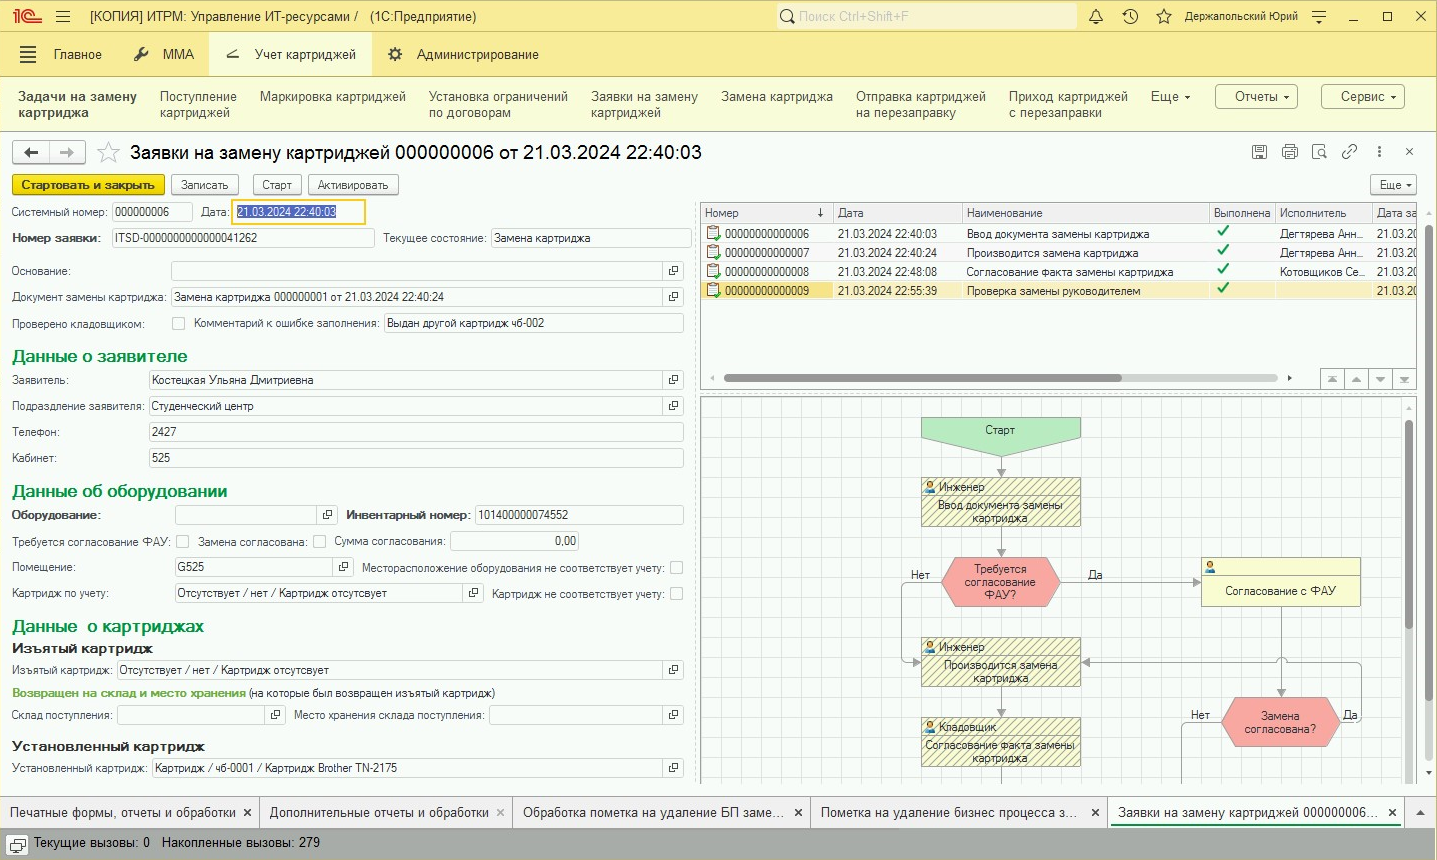
\includegraphics[width=14cm]{pictures/process.png}
    % %     % \caption{}  \label{pic_label}
    % % \end{figure}

